\section{Results}
\label{sec:results}




\begin{figure}
\begin{tabular}{ l l}
  \hspace{3.5cm}(a) & \hspace{7cm}(b)\\
\end{tabular}\\
\resizebox{6in}{!}{
  \begin{tabular}{c c}
  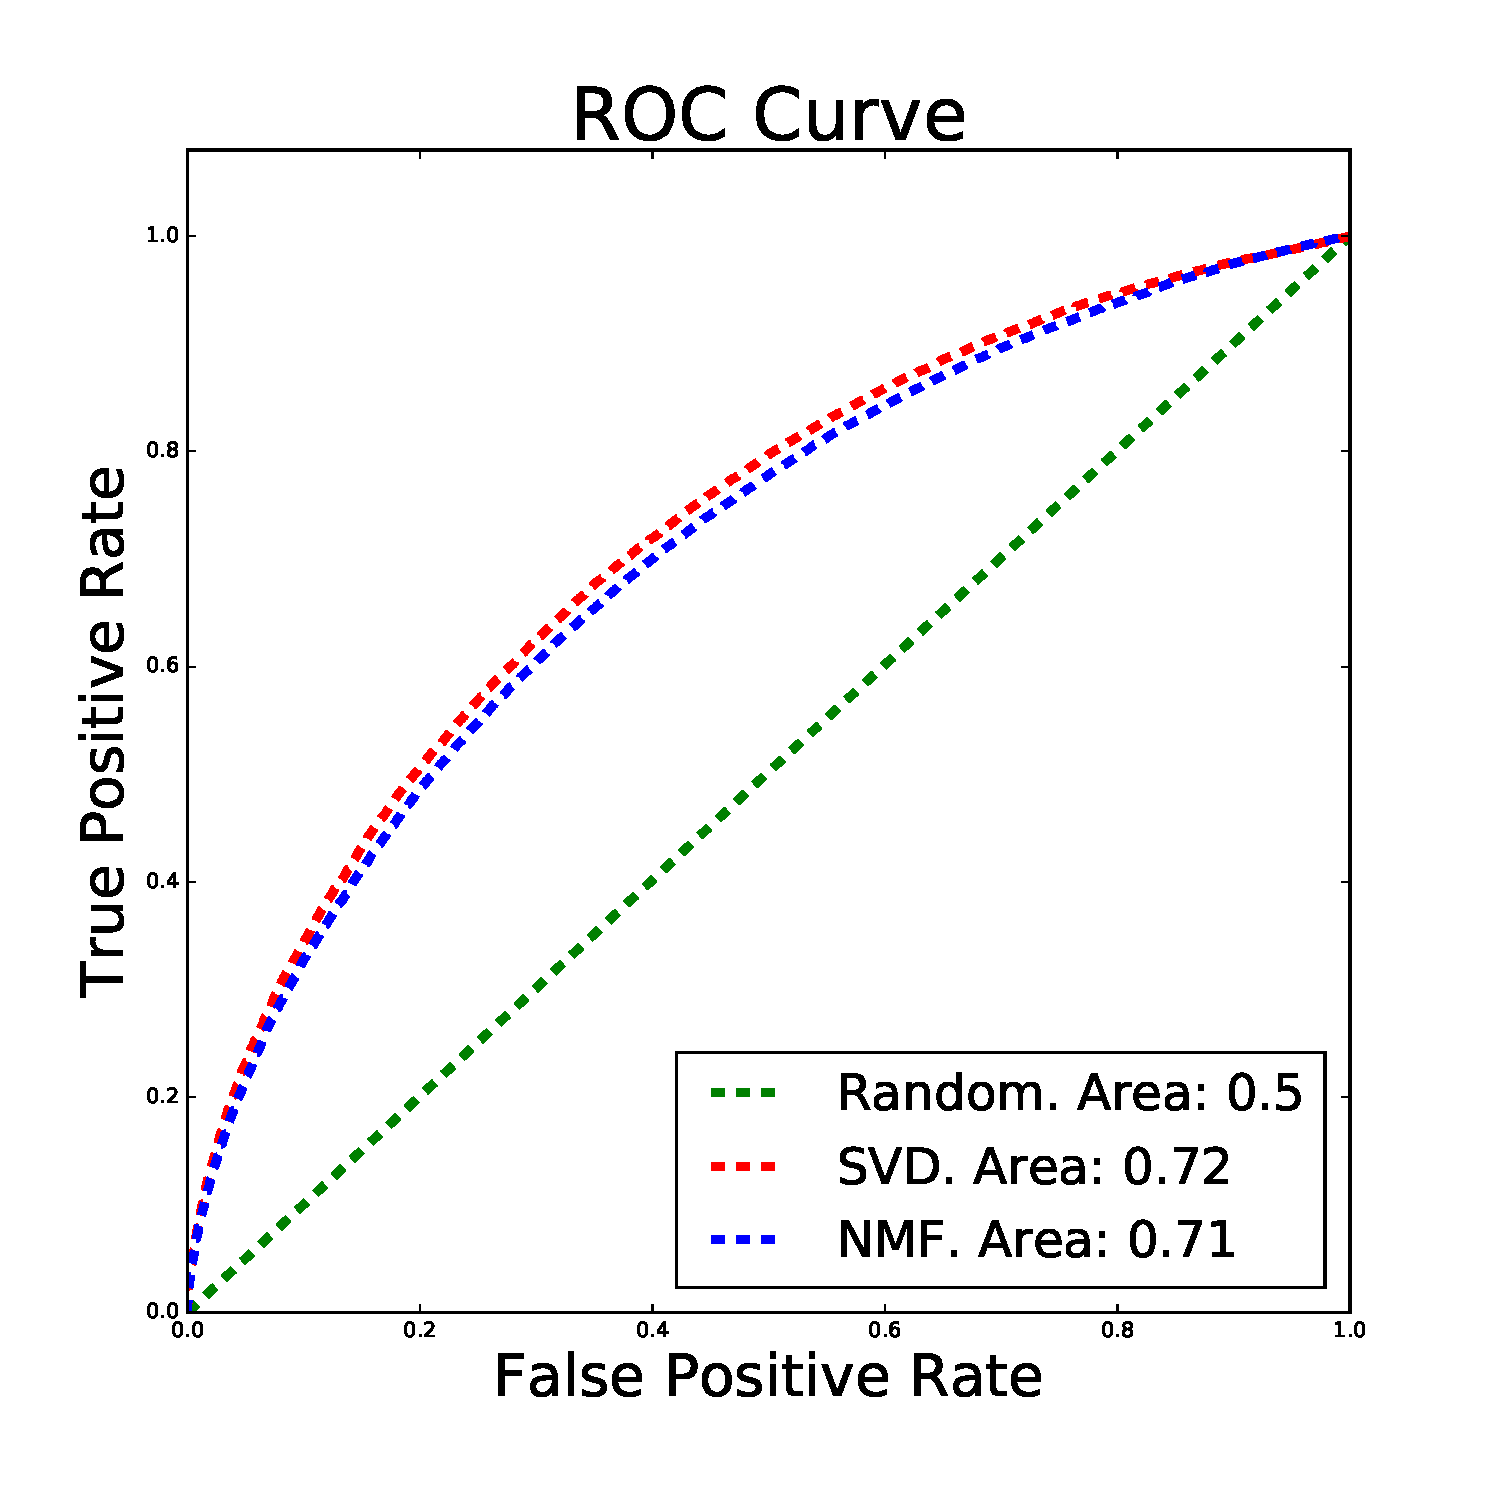
\includegraphics{figures/roc_curve.pdf} 
  &  
  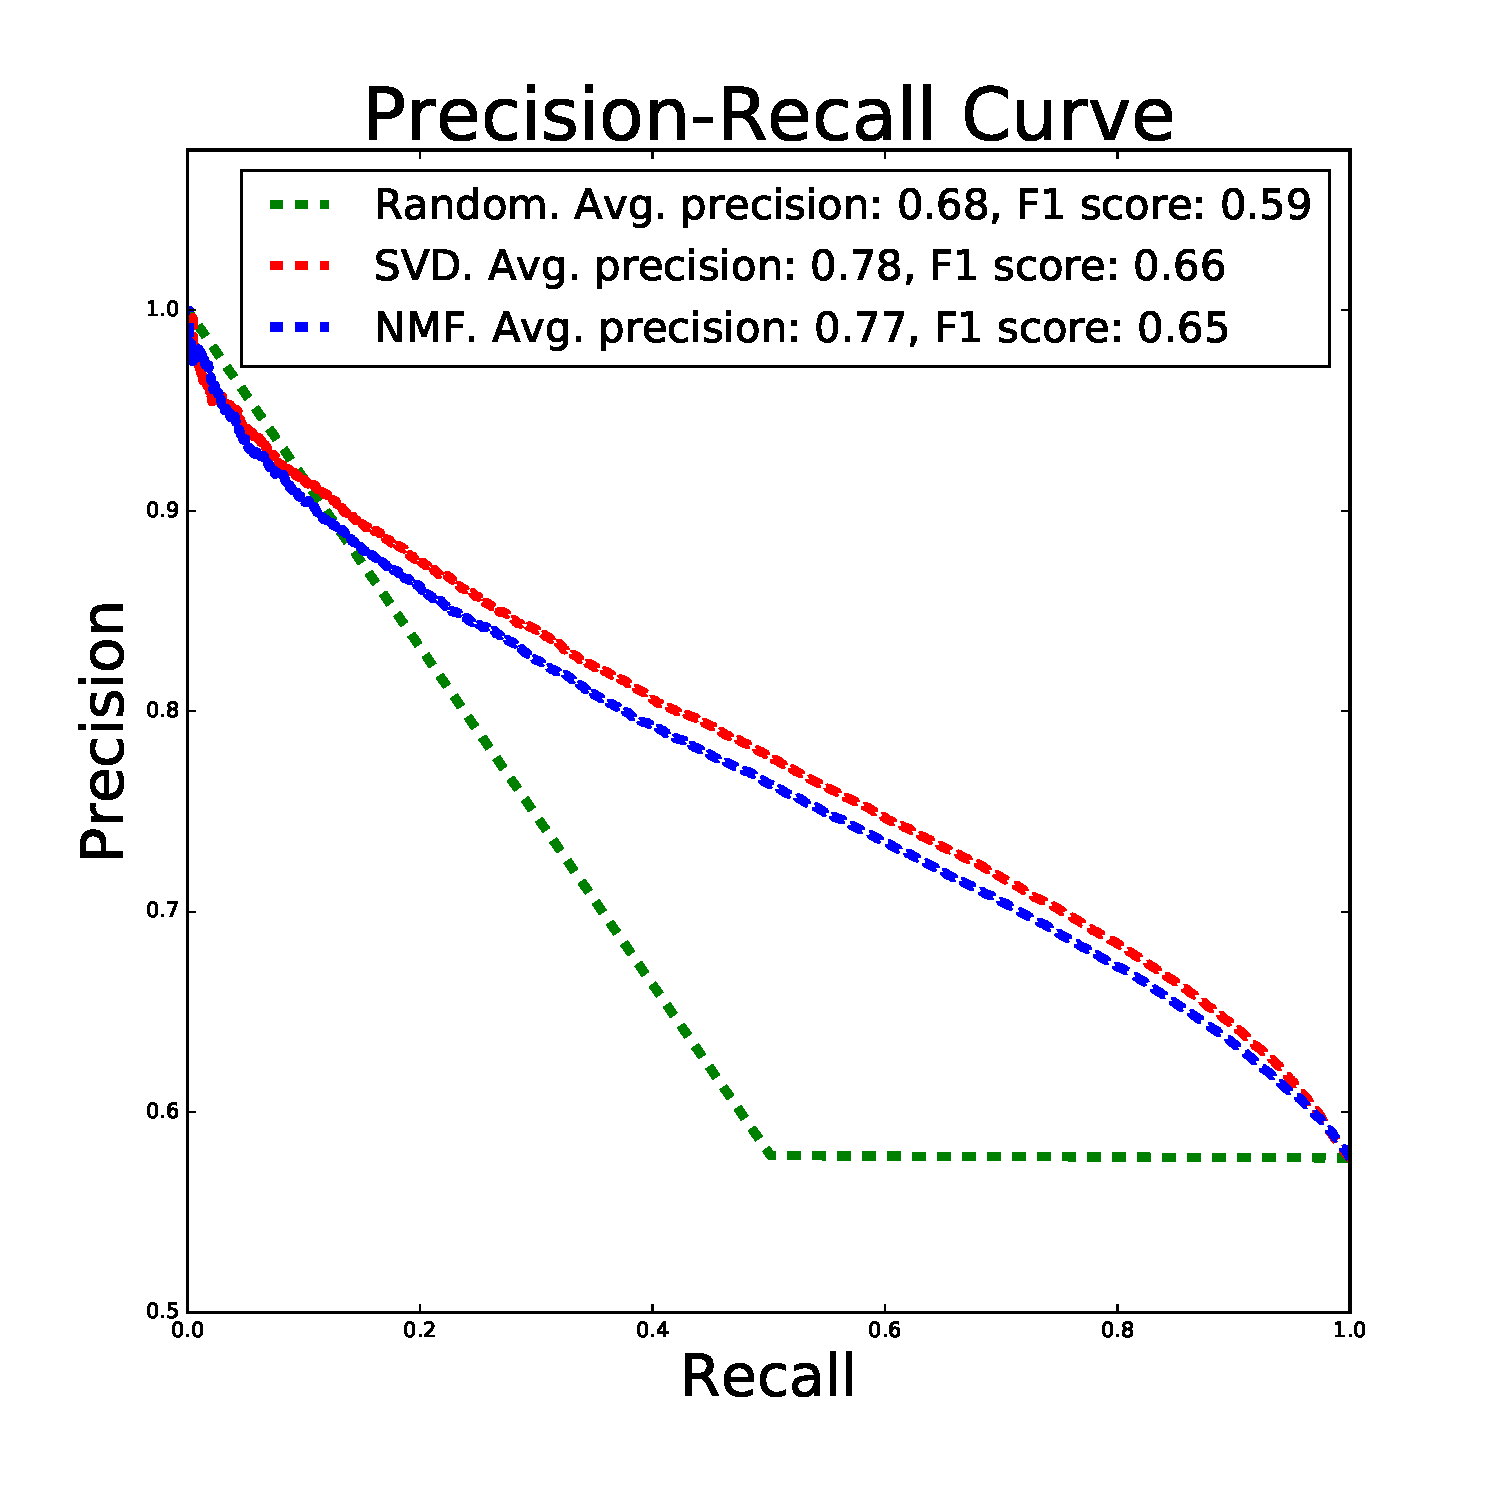
\includegraphics{figures/precision_recall_curve.pdf} \\
\end{tabular}
}
\caption{Matrix Factorization Results: (a) ROC Curve, (b) Precision Recall Curve}
\label{fig:matrix_curves}  
\end{figure}


To evaluate our prediction performance for the neighborhood models, we used two accepted metrics: one is RMSE, which was used in the \textit{Netflix Prize} competition, and the the winner, Yehuda Koren, demonstrated later in a different paper that RMSE is a good measurement for recommender systems providing "top K recommendations"~\cite{koren2008factorization}. They witnessed that small improvements in the RMSE translated into significant improvements in the quality of the top K items in the recommended list. The second metric is called Normalized Discounted Cumulative Gain (NDCG), and it is used in many recommendation system studies to score the relevance of the top K items in the list. This metric allows the relevance scores of the items to be real numbers, so we have used our predicted ratings to sort the recommended movie list. The algorithm we used was implemented by Mathieu Blondel~\cite{letorMetrics}. We calculated NDCG@k for $k=\{5, 10, 15, 20\}$, since these numbers represent a reasonable length of movie recommendation list.

We present the results of ratings prediction using cosine similarity in the form of RMSE, averaged on the 10-folds cross validation runs, for each of the representative 10 users individually. 
The RMSE is plotted as a function of the number of similar users we have taken into account in the prediction. 
We can see in Figure~\ref{fig:user_similarity} that the RMSE decreases as additional similar users are added, reaching a minimum of 0.84.
Furthermore, we see that beyond the point of six users, the average RMSE curve plateaus, and the RMSE improvement curve is roughly zero.
As we ran the experiments for higher number of similar users, we saw that beyond roughly 64 similar users the addition of users had an adverse effect on prediction, as RMSE increased for larger numbers of similar users. We did not extend our figure beyond 16 users, for esthetic reasons. 

The results of ratings prediction using K-means clustering are presented in the form of NDCG@k averaged on the 10-folds cross validation runs, for each of the representative 10 users individually. For two users we have less than 100 ratings so each cross-validation run resulted in less than 10 ranked reviews; therefore, we report only NDCG@k, k=5 for those users. In Figure~\ref{fig:ndcg} the NDCG@k is plotted for each user, when the users are sorted according to three different features: \blackone The number of the user ratings \blacktwo The average of the user ratings \blackthree The standard deviation of the user ratings. We can see that for most users and most k the NDCG is above 0.7. The quality of prediction is a trend within each user, it's either high for all k, or low for all of them. As for k, when averaging on all the users per each k individually, we get the following: 0.717, 0.719, 0.749 and 0.785 for k=5,10,15,20 respectively. This is a linear increase in prediction quality with the length of the recommendation list. The Number of ratings and the ratings standard deviation don't seem to improve the prediction quality as the average NDCG doesn't increase or decrease together with them. We do see an improvement in the average NDCG for users with higher ratings average. Another thing to note here is that even for the two users with a low number of ratings (less than 100), we are able to achieve a good NDCG@k for k=5, again supporting the observation that the ratings number is not a factor in the prediction quality, and we can predict even for users with a short ratings history. 


Finally, Figure~\ref{fig:matrix_curves} shows the results of the binary prediction using matrix factorization. 
We see that both SVD and NMF achieve similar performance, SVD does slightly better by achieving an F1 score of 0.66, average precision of 0.78 and the AUC for the ROC curve is 0.72.
